\documentclass[10pt, a4paper]{article}

\usepackage{ctex}
\usepackage{xeCJK}
\usepackage{caption}
\usepackage{geometry}
\geometry{
    left = 0.6in,
    right = 0.6in,
    top = 0.8in,
    bottom = 1.0in
}
\usepackage{amssymb}
\usepackage{amsbsy}
\usepackage{amsmath}
\usepackage{xcolor}
\usepackage{mathrsfs}
\usepackage{graphicx}
\usepackage{pifont}
\usepackage{tikz}
\usepackage{tasks}
\settasks{
    label = \Alph*. ,
    label-width = 16pt
}

\newcommand{\Title}[3]{
    \begin{center}
        \Large \textbf{中国电子学会 #1~年~#2~月 Scratch~#3级考试}
    \end{center}
}
\newcommand{\TimeAndName}[1]{
    \begin{center}
        考试时间:~#1~ 分钟 \qquad\qquad\qquad\qquad 姓名:\underline{\quad\quad\quad\quad}
    \end{center}
}
\pagestyle{empty}
\begin{document}
    \Title{2020}{9}{一}
    
    \TimeAndName{60}
    
    {\noindent\heiti 第一部分、单选题(共 25 题,每题 2 分,共50分.)}

    \begin{enumerate}
        % 1
        \item 下面哪个积木能够调节左右声道的音量?(\qquad)
        \begin{tasks}(4)
            \task 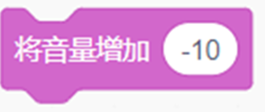
\includegraphics[width=.1\textwidth]{1a.png}
            \task 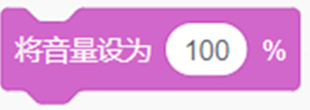
\includegraphics[width=.12\textwidth]{1b.png}
            \task 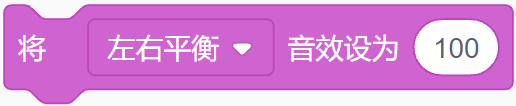
\includegraphics[width=.18\textwidth]{1c.png}
            \task 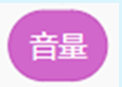
\includegraphics[width=.05\textwidth]{1d.png}
        \end{tasks}

        % 2
        \item 当我们进行数学计算时,需要用到下面哪个模块中的积木?(\qquad)
        \begin{tasks}(4)
            \task 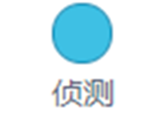
\includegraphics[width=.05\textwidth]{2a.png}
            \task 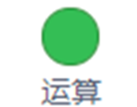
\includegraphics[width=.05\textwidth]{2b.png}
            \task 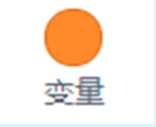
\includegraphics[width=.05\textwidth]{2c.png}
            \task 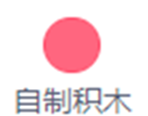
\includegraphics[width=.05\textwidth]{2d.png}
        \end{tasks}

        % 3
        \item 下面哪个区域是“背景区”?(\qquad)
        \begin{tasks}(4)
            \task A
            \task B
            \task C
            \task D
        \end{tasks}

        % 4
        \item 以下哪组积木块不能实现小猫最终方向为130度?(\qquad)
        \begin{tasks}(4)
            \task 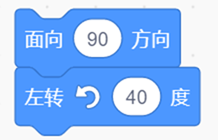
\includegraphics[width=.12\textwidth]{4a.png}
            \task 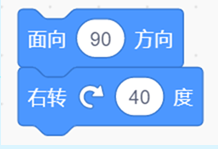
\includegraphics[width=.12\textwidth]{4b.png}
            \task 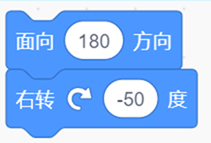
\includegraphics[width=.12\textwidth]{4c.png}
            \task 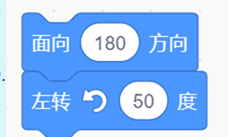
\includegraphics[width=.14\textwidth]{4d.png}
        \end{tasks}

        \begin{figure}[htbp]
            \centering
            \begin{minipage}[t]{.2\textwidth}
                \centering
                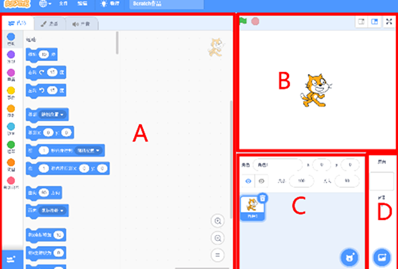
\includegraphics[width=1\textwidth]{3.png}
                \caption*{第3题}
            \end{minipage}
            \begin{minipage}[t]{.18\textwidth}
                \centering
                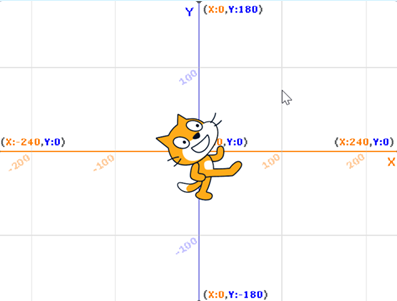
\includegraphics[width=\textwidth]{5.png}
                \caption*{第5题}
            \end{minipage}
            \begin{minipage}[t]{.2\textwidth}
                \centering
                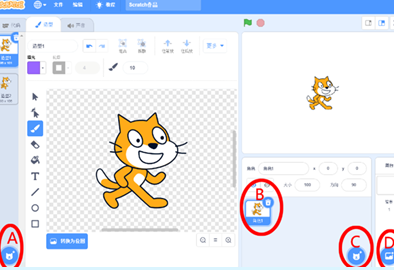
\includegraphics[width=\textwidth]{6.png}
                \caption*{第6题}
            \end{minipage}
            \begin{minipage}[t]{.38\textwidth}
                \centering
                \begin{minipage}[t]{.5\textwidth}
                    \centering
                    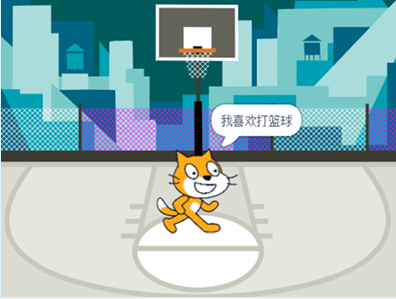
\includegraphics[width=\textwidth]{8-1.png}
                \end{minipage}
                \begin{minipage}[t]{.48\textwidth}
                    \centering
                    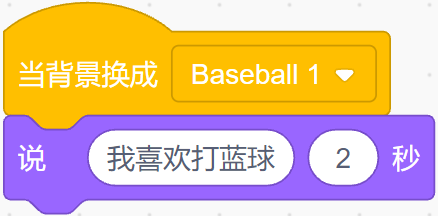
\includegraphics[width=\textwidth]{8-2.png}
                \end{minipage}
                \caption*{第8题}
            \end{minipage}
        \end{figure}

        % 5
        \item 小猫的初始方向和鼠标的位置如上图所示,下面哪个积木可以让角色面向正右方?(\qquad)
        \begin{tasks}(4)
            \task 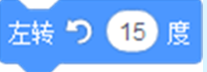
\includegraphics[width=.12\textwidth]{5a.png}
            \task 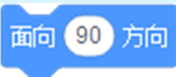
\includegraphics[width=.12\textwidth]{5b.png}
            \task 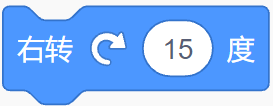
\includegraphics[width=.12\textwidth]{5c.png}
            \task 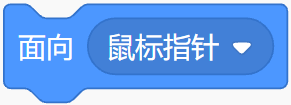
\includegraphics[width=.12\textwidth]{5d.png}
        \end{tasks}

        % 6
        \item 使用上图中哪个按钮可以添加新角色?(\qquad)
        \begin{tasks}(4)
            \task A
            \task B
            \task C
            \task D
        \end{tasks}

        % 7
        \item 现在音量为100,不改变下面积木参数,哪个积木可以上音量小一点?(\qquad)
        \begin{tasks}(4)
            \task 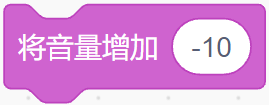
\includegraphics[width=.13\textwidth]{7a.png}
            \task 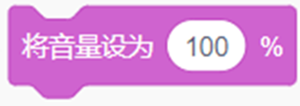
\includegraphics[width=.15\textwidth]{7b.png}
            \task 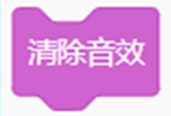
\includegraphics[width=.08\textwidth]{7c.png}
            \task 
\includegraphics[width=.07\textwidth]{7d.png}
        \end{tasks}
           
        % 8
        \item 现在有三个背景:"Mountain"、"Basketball 1"、“Colorful City”,下面哪个程序能够实现背景按顺序切换,在切换到Basketball 1背景时,小猫说“我喜欢打篮球2秒”,切换其他背景时小猫都不说话?(\qquad)
        \begin{tasks}(4)
            \task 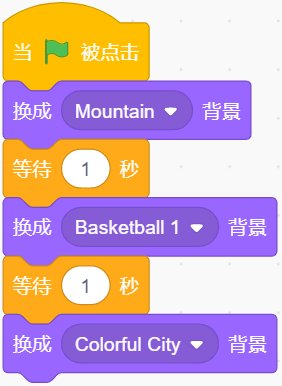
\includegraphics[width=.12\textwidth]{8a.png}
            \task 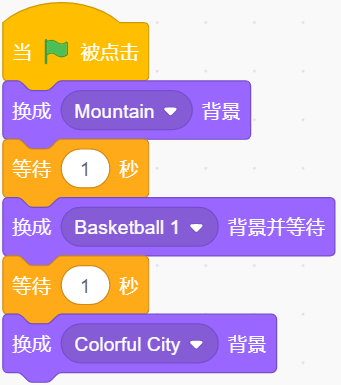
\includegraphics[width=.14\textwidth]{8b.png}
            \task 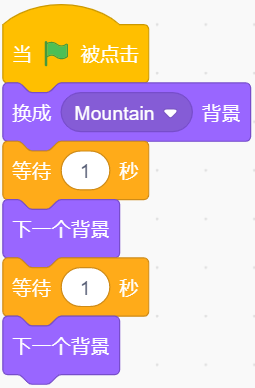
\includegraphics[width=.1\textwidth]{8c.png}
            \task 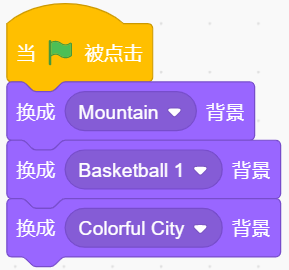
\includegraphics[width=.15\textwidth]{8d.png}
        \end{tasks}

        \newpage
        % 9
        \item 小猫初始方向如图1,小猫看到一个香蕉如图2,下面哪段程序执行后,可以让小猫拿到香蕉后如图3?(\qquad)
        \begin{tasks}(4)
            \task 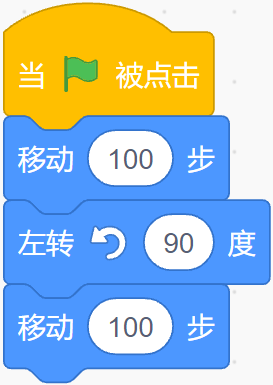
\includegraphics[width=.12\textwidth]{9a.png}
            \task 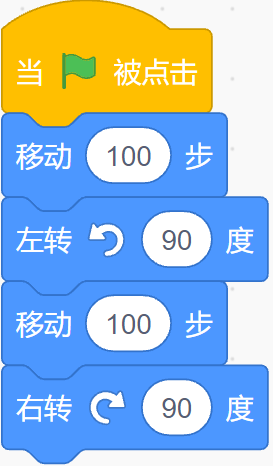
\includegraphics[width=.1\textwidth]{9b.png}
            \task 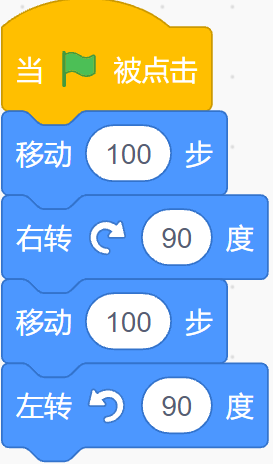
\includegraphics[width=.1\textwidth]{9c.png}
            \task 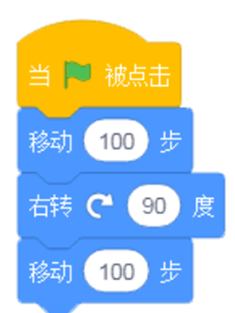
\includegraphics[width=.12\textwidth]{9d.png}
        \end{tasks}

       % 10
       \item 点击下面哪个图标可以使舞台区最大化?(\qquad)
       \begin{tasks}(4)
           \task 
\includegraphics[width=.04\textwidth]{10a.png}
           \task 
\includegraphics[width=.05\textwidth]{10b.png}
           \task 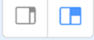
\includegraphics[width=.09\textwidth]{10c.png}
           \task 
\includegraphics[width=.05\textwidth]{10d.png}
       \end{tasks}

        % 11
        \item 现在的音量为50,不改变积木的参数,下面哪个积木可以让音量大一些?(\qquad)
        \begin{tasks}(4)
            \task 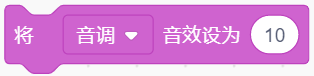
\includegraphics[width=.15\textwidth]{11a.png}
            \task 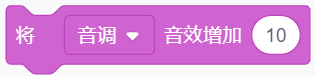
\includegraphics[width=.15\textwidth]{11b.png}
            \task 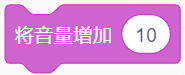
\includegraphics[width=.1\textwidth]{11c.png}
            \task 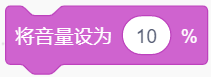
\includegraphics[width=.12\textwidth]{11d.png}
        \end{tasks}
        
        % 12
        \item 每个方格的边长是30,下面哪个程序可以让青蛙抓住蝴蝶?(\qquad)
        \begin{tasks}(4)
            \task 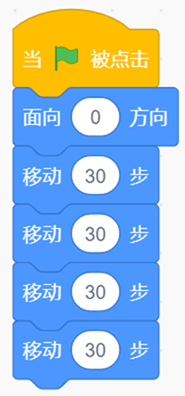
\includegraphics[width=.1\textwidth]{12a.png}
            \task 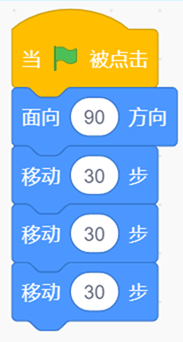
\includegraphics[width=.11\textwidth]{12b.png}
            \task 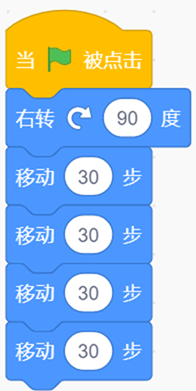
\includegraphics[width=.1\textwidth]{12c.png}
            \task 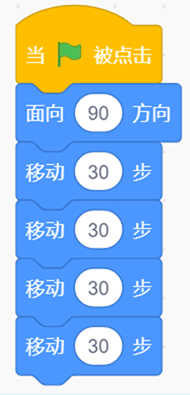
\includegraphics[width=.1\textwidth]{12d.png}
        \end{tasks}

        \begin{figure}[htbp]
            \centering
            \begin{minipage}[t]{.4\textwidth}
                \centering
                \begin{minipage}[t]{.17\textwidth}
                    \centering
                    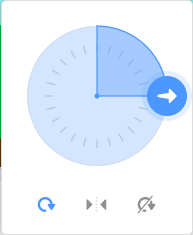
\includegraphics[width=\textwidth]{9-1.png}
                \end{minipage}
                \begin{minipage}[t]{.4\textwidth}
                    \centering
                    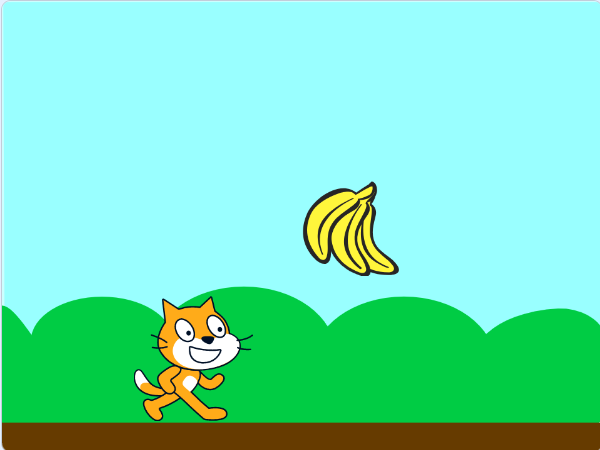
\includegraphics[width=1\textwidth]{9-2.png}
                \end{minipage}
                \begin{minipage}[t]{.4\textwidth}
                    \centering
                    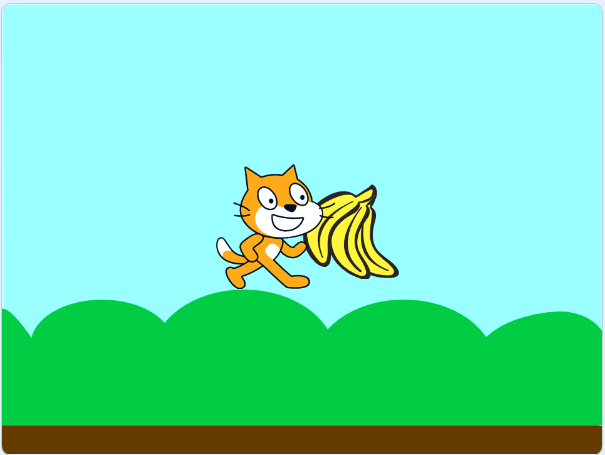
\includegraphics[width=1\textwidth]{9-3.png}
                \end{minipage}
                \caption*{第9题}
            \end{minipage}
            \begin{minipage}[t]{.23\textwidth}
                \centering
                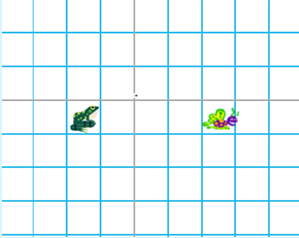
\includegraphics[width=.8\textwidth]{12.png}
                \caption*{第12题}
            \end{minipage}
            \begin{minipage}[t]{.09\textwidth}
                \centering
                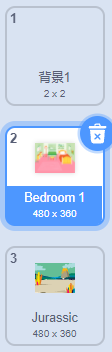
\includegraphics[width=.6\textwidth]{13.png}
                \caption*{第13题}
            \end{minipage}
            \begin{minipage}[t]{.23\textwidth}
                \centering
                \includegraphics[width=.8\textwidth]{14.png}
                \caption*{第14题}
            \end{minipage}
        \end{figure}

        % 13
        \item 如上图,当前背景是第二个背景,不改变积木参数,下面哪个积木,可以换成下一个背景?(\qquad)
        \begin{tasks}(4)
            \task \includegraphics[width=.08\textwidth]{13a.png}
            \task \includegraphics[width=.12\textwidth]{13b.png}
            \task \includegraphics[width=.08\textwidth]{13c.png}
            \task \includegraphics[width=.12\textwidth]{13d.png}
        \end{tasks}

        % 14
        \item 如上图,下面哪个积木可以让角色面向正上方?(\qquad)
        \begin{tasks}(4)
            \task \includegraphics[width=.08\textwidth]{14a.png}
            \task \includegraphics[width=.1\textwidth]{14b.png}
            \task \includegraphics[width=.1\textwidth]{14c.png}
            \task \includegraphics[width=.1\textwidth]{14d.png}
        \end{tasks}
    
        \item 下面哪个程序不能让角色换成第三个造型?(\qquad)
        
        \begin{minipage}{.1\textwidth}
            \centering
            \includegraphics[width=0.8\textwidth]{15.png}
        \end{minipage}
        \begin{minipage}{.78\textwidth}
            \begin{tasks}(4)
                \task \includegraphics[width=.14\textwidth]{15a.png}
                \task \includegraphics[width=.14\textwidth]{15b.png}
                \task \includegraphics[width=.14\textwidth]{15c.png}
                \task \includegraphics[width=.14\textwidth]{15d.png}
            \end{tasks}
        \end{minipage}
        
        % 16
        \item 小猫在舞台上左右来回走,使用下面哪种旋转方式量合适?(\qquad)
        \begin{tasks}(4)
            \task \includegraphics[width=.08\textwidth]{16a.png}
            \task \includegraphics[width=.08\textwidth]{16b.png}
            \task \includegraphics[width=.08\textwidth]{16c.png}
            \task \includegraphics[width=.08\textwidth]{16d.png}
        \end{tasks}

        % 17
        \item 下面哪个积木可以获取当前背景的名称?(\qquad)
        \begin{tasks}(4)
            \task \includegraphics[width=.12\textwidth]{17a.png}
            \task \includegraphics[width=.12\textwidth]{17b.png}
            \task \includegraphics[width=.12\textwidth]{17c.png}
            \task \includegraphics[width=.12\textwidth]{17d.png}
        \end{tasks}

        % 18
        \item 如下图所示,图中“?”位置,应该填入的图形是?(\qquad)
        \begin{tasks}(4)
            \task \includegraphics[width=.05\textwidth]{18a.png}
            \task \includegraphics[width=.05\textwidth]{18b.png}
            \task \includegraphics[width=.05\textwidth]{18c.png}
            \task \includegraphics[width=.05\textwidth]{18d.png}
        \end{tasks}

        % 19
        \item 小明想实现小女孩跳芭蕾舞的动画,但程序执行后没有看到小女孩动作变化,用下面哪个方法可以帮助他实现正确的效果?(\qquad)
        \begin{tasks}(2)
            \task 造型太少,需要多复制几个造型
            \task 在“下一个造型”积木中间插入“等待1秒”积木
            \task 上下拖动造型,重新排序
            \task 造型太多,删除一些
        \end{tasks}

        \begin{figure}[htbp]
            \centering
            \begin{minipage}[t]{.22\textwidth}
                \centering
                \includegraphics[width=\textwidth]{18.png}
                \caption*{第18题}
            \end{minipage}
            \begin{minipage}[t]{.21\textwidth}
                \centering
                \includegraphics[width=\textwidth]{19.png}
                \caption*{第19题}
            \end{minipage}
            \begin{minipage}[t]{.23\textwidth}
                \centering
                \includegraphics[width=\textwidth]{20.png}
                \caption*{第20题}
            \end{minipage}
            \begin{minipage}[t]{.27\textwidth}
                \centering
                \includegraphics[width=\textwidth]{21.png}
                \caption*{第21题}
            \end{minipage}
        \end{figure}

        % 20
        \item 点击上图中哪个按钮可以绘制新背景?(\qquad)
        \begin{tasks}(4)
            \task A
            \task B
            \task C
            \task D
        \end{tasks}

        % 21
        \item 上图中哪个按钮可以实现填充颜色?(\qquad)
        \begin{tasks}(4)
            \task \includegraphics[width=.04\textwidth]{21a.png}
            \task \includegraphics[width=.04\textwidth]{21b.png}
            \task \includegraphics[width=.04\textwidth]{21c.png}
            \task \includegraphics[width=.04\textwidth]{21d.png}
        \end{tasks}

        % 22
        \item 下面哪个积木可以让角色左右运动时不倒立?(\qquad)
        \begin{tasks}(4)
            \task \includegraphics[width=.12\textwidth]{22a.png}
            \task \includegraphics[width=.15\textwidth]{22b.png}
            \task \includegraphics[width=.12\textwidth]{22c.png}
            \task \includegraphics[width=.18\textwidth]{22d.png}
        \end{tasks}

        % 23
        \item 下图中哪个按钮可以上传声音?(\qquad)
        
        \begin{minipage}{.15\textwidth}
            \centering
            \includegraphics[width=\textwidth]{23.png}
        \end{minipage}
        \begin{minipage}{.78\textwidth}
            \begin{tasks}(4)
                \task A
                \task B
                \task C
                \task D
            \end{tasks}
        \end{minipage}

        % 24
        \item 小明家楼上有3层,楼下有2层,这栋楼一共多少层?(\qquad)
        \begin{tasks}(4)
            \task 3
            \task 2
            \task 6
            \task 5
        \end{tasks}
        
        % 25
        \item 方格的边长为30,下面哪个程序可以让青蛙沿着箭头抓到蝴蝶?(\qquad)
        \begin{tasks}(4)
            \task \includegraphics[width=.1\textwidth]{25a.png}
            \task \includegraphics[width=.08\textwidth]{25b.png}
            \task \includegraphics[width=.12\textwidth]{25c.png}
            \task \includegraphics[width=.12\textwidth]{25d.png}
        \end{tasks}
    \end{enumerate}

    \begin{figure}[htbp]
        \centering
        \begin{minipage}[t]{.23\textwidth}
            \centering
            \includegraphics[width=\textwidth]{25.png}
            \caption*{第25题}
        \end{minipage}
        \begin{minipage}[t]{.23\textwidth}
            \centering
            \begin{minipage}[t]{.23\textwidth}
                \centering
                \includegraphics[width=\textwidth]{28-1.png}
            \end{minipage}
            \begin{minipage}[t]{.7\textwidth}
                \centering
                \includegraphics[width=\textwidth]{28-2.png}
            \end{minipage}
            \caption*{第28题}
        \end{minipage}
        \begin{minipage}[t]{.23\textwidth}
            \centering
            \includegraphics[width=\textwidth]{30.png}
            \caption*{第30题}
        \end{minipage}
        \begin{minipage}[t]{.13\textwidth}
            \centering
            \includegraphics[width=\textwidth]{33.png}
            \caption*{第33题}
        \end{minipage}
    \end{figure}

    {\noindent\heiti 第二部分、判断题(共 10 题,每题 2 分,共20分.)}
    \begin{enumerate}
        \setcounter{enumi}{25}
        % 26
        \item 如图\includegraphics[width=.12\textwidth]{26.png}所示,积木的运算结果是12.(\qquad)

        %27
        \item 点击图\includegraphics[width=.02\textwidth]{27-1.png}或图\includegraphics[width=.04\textwidth]{27-2.png}中的按钮,都可以从音乐库中“选择一个声音”.(\qquad)
        
        %28
        \item 上面舞台的程序可以播放“Dance Around”这首音乐.(\qquad)
  
        %29
        \item 鼠标移到图\includegraphics[width=.03\textwidth]{29-1.png}按钮,在弹出的上拉列表中,点击\includegraphics[width=.025\textwidth]{29-2.png}按钮可以绘制新角色.(\qquad)
        
        %30
        \item 改变上图中“大小”的数值,可以调整“Bear”角色的大小.(\qquad)

        %31
        \item 使用积木\includegraphics[width=.08\textwidth]{31.png},可以让角色倒退.(\qquad)
        
        %32
        \item 只有删除了当前背景才可以添加新背景.(\qquad)
        
         %33
         \item 如上图,点击红框中的按钮都可以删除角色.(\qquad)
        
         %34
         \item 点击图\includegraphics[width=.03\textwidth]{34-1.png}或图\includegraphics[width=.03\textwidth]{34-2.png}按钮都可以可以“选择一个背景”.(\qquad)
         
         %35
         \item 在编写程序时,如果不小心删除了积木,就没办法撤销删除操作.(\qquad)
    \end{enumerate}

    \newpage
    {\noindent\heiti 第三部分、编程题(共 2 题,共30分.)}
    \begin{enumerate}
        \setcounter{enumi}{35}
        
        %36
        \item 小鸡与鸭妈妈拥抱:
 
        1. 准备工作
        \begin{tasks}[label = (\arabic*)]
            \task 背景:Farm;
            \task 角色:Chick、Duck.
        \end{tasks}
        2. 功能实现
        \begin{tasks}[label = (\arabic*)]
            \task 角色的初始位置、方向和造型如图所示;
            \task 点击绿旗Chick向右走去,边走边切换造型;
            \task 点击绿旗Duck向左走去;
            \task 2个动物拥抱后停止移动,Duck播放声音"Duck"。
        \end{tasks}
        \begin{figure}[htbp]
            \centering
            \includegraphics[width=.4\textwidth]{36.png}
        \end{figure}
            
        % 37
        \item 字母AB点头问好:
        
        1. 准备工作
        \begin{tasks}[label = (\arabic*)]
            \task 背景:Chalkboard;
            \task 角色:Glow-B,Glow-A;
        \end{tasks}
        2. 功能实现
        \begin{tasks}[label = (\arabic*)]
            \task 点击绿旗,字母B和字母A初始化位置,如图1所示;
            \task 点击绿旗,字母B向右旋转一个角度,一步一步移到黑板上,点头两次,如图2、图3所
            示;
            \task 点击绿旗,等到字母B点头后,字母A向左一步一步移到到黑板上,点头两次,如图4、
            图5所示。
        \end{tasks}
        \begin{figure}[htbp]
            \centering
            \begin{minipage}[t]{.18\textwidth}
                \centering
                \includegraphics[width=\textwidth]{37-1.png}
                \caption*{图1}
            \end{minipage}
            \begin{minipage}[t]{.18\textwidth}
                \includegraphics[width=\textwidth]{37-2.png}
                \caption*{图2}
            \end{minipage}
            \begin{minipage}[t]{.18\textwidth}
                \centering
                \includegraphics[width=\textwidth]{37-3.png}
                \caption*{图3}
            \end{minipage}
            \begin{minipage}[t]{.18\textwidth}
                \includegraphics[width=\textwidth]{37-4.png}
                \caption*{图4}
            \end{minipage}
            \begin{minipage}[t]{.18\textwidth}
                \centering
                \includegraphics[width=\textwidth]{37-5.png}
                \caption*{图5}
            \end{minipage}
        \end{figure}
    \end{enumerate}
\end{document}